\section{USER INTERFACE DESIGN}

This chapter illustrates the user interface mockups. Specifically, it revisits 
the mockups originally presented in the RASD, supplementing them with additional 
screens to provide a more design-oriented perspective. \\

\noindent Displayed below is the initial screen encountered upon launching the mobile application. As can be observed, this 
interface offers the option to log in (located at the top) or to proceed in Guest Mode 
(shown at the bottom). As previously stated, Guest Mode is restricted; consequently, 
users operating in this mode are limited solely to searching for paths within the BBP 
system database.

\begin{figure}[H]
    \centering
    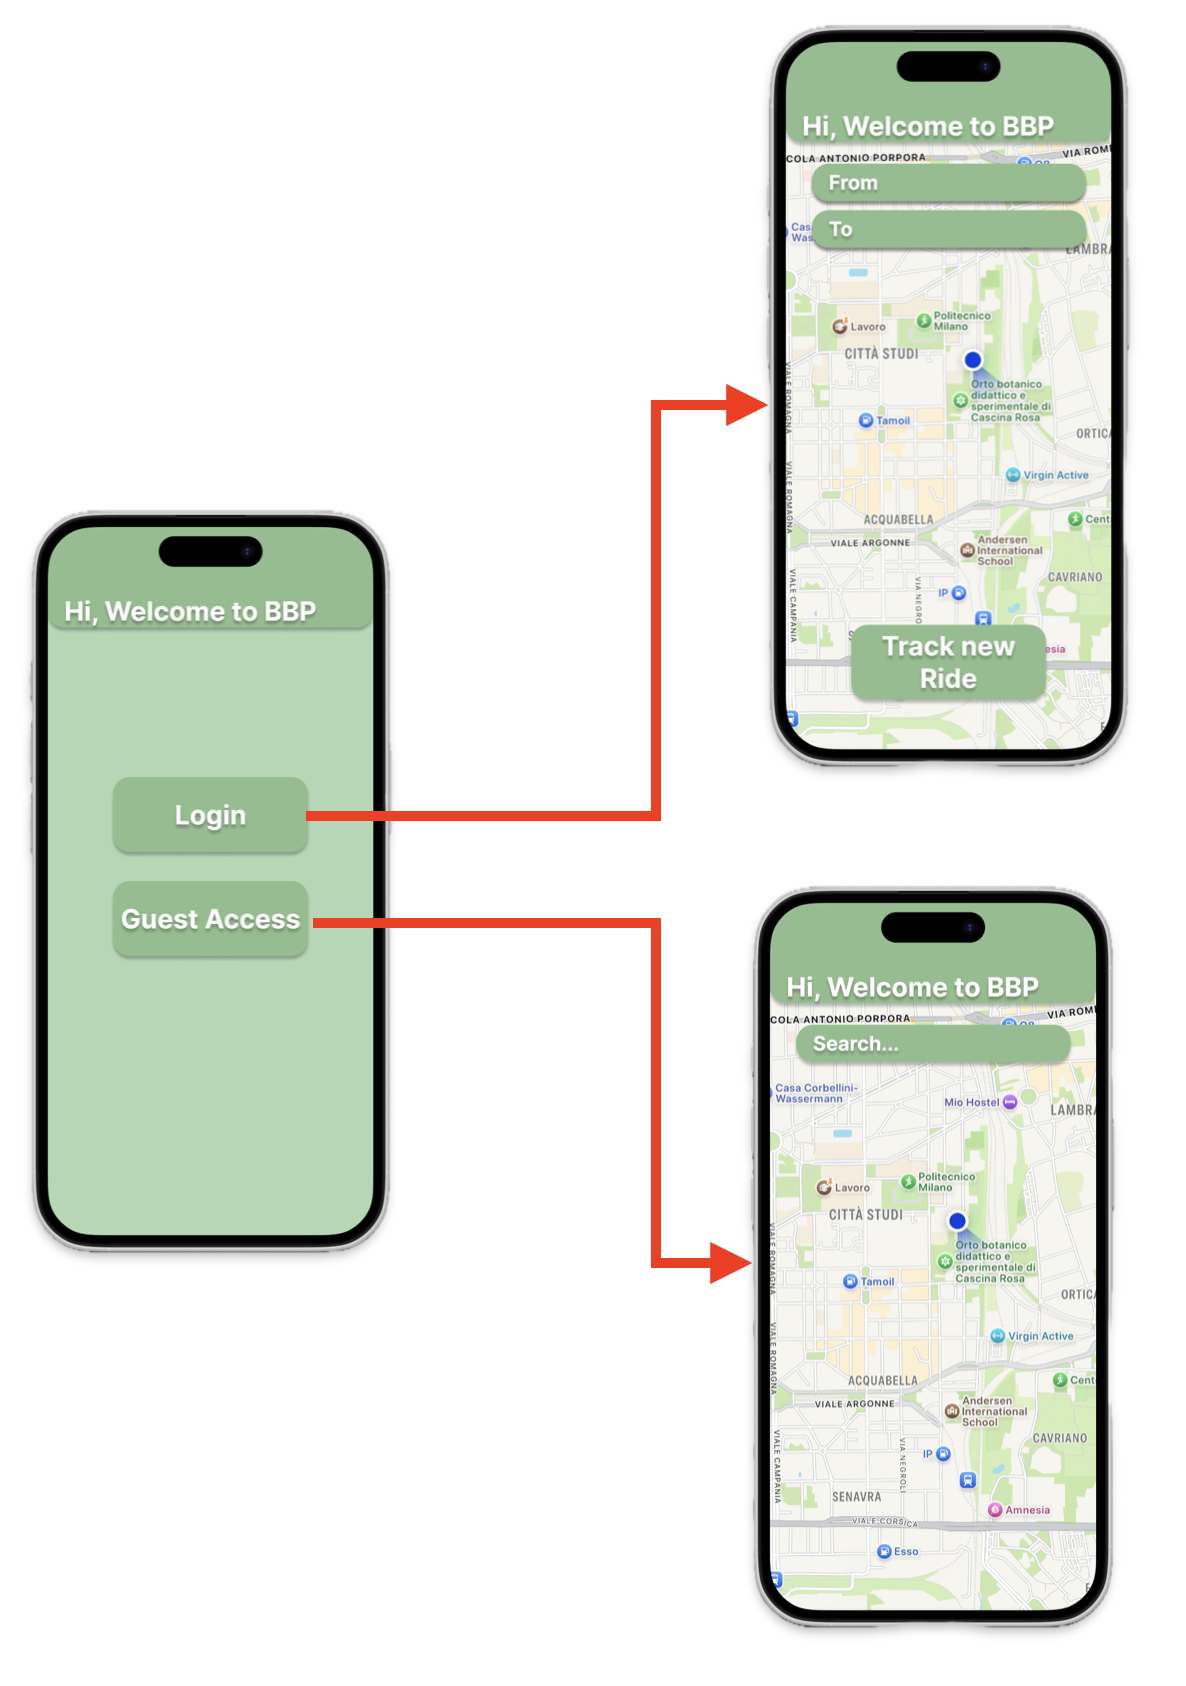
\includegraphics[width=0.5\textwidth]{images/prototype1.png}
    \caption{Homepage screen mockup}
    \label{fig:startup_mockup}
\end{figure}    

\noindent The following screens present the general workflow, illustrating the two tracking 
alternatives available for recording a new ride: automatic and manual. Specifically, 
upon clicking 'Track New Ride', the user is given the option to select the data acquisition 
mode. \\

\noindent If manual mode is selected (illustrated at the top), the user is presented with 
a form to sequentially enter each street (or street segment) and its corresponding status. 
Upon completing this process and confirming, the user is directed to a preview screen.\\

\noindent A similar screen is also displayed to users who, after selecting automated mode, 
decide to terminate the session (or when the system detects inactivity and automatically 
interrupts data acquisition). \\

\noindent In either scenarios, once on the preview screen, the user can 
further refine the manually entered or automatically detected data. In the second case, the refinement is mandatory. Finally, the user can choose 
to press 'Exit' to discard the collected data or 'Save' to store the acquired data locally. 
Should the latter option be selected, the user must be offered the choice to either publish 
the path or keep it private, making it viewable solely by them within their personal records log.\\

\begin{figure}[H]
    \centering
    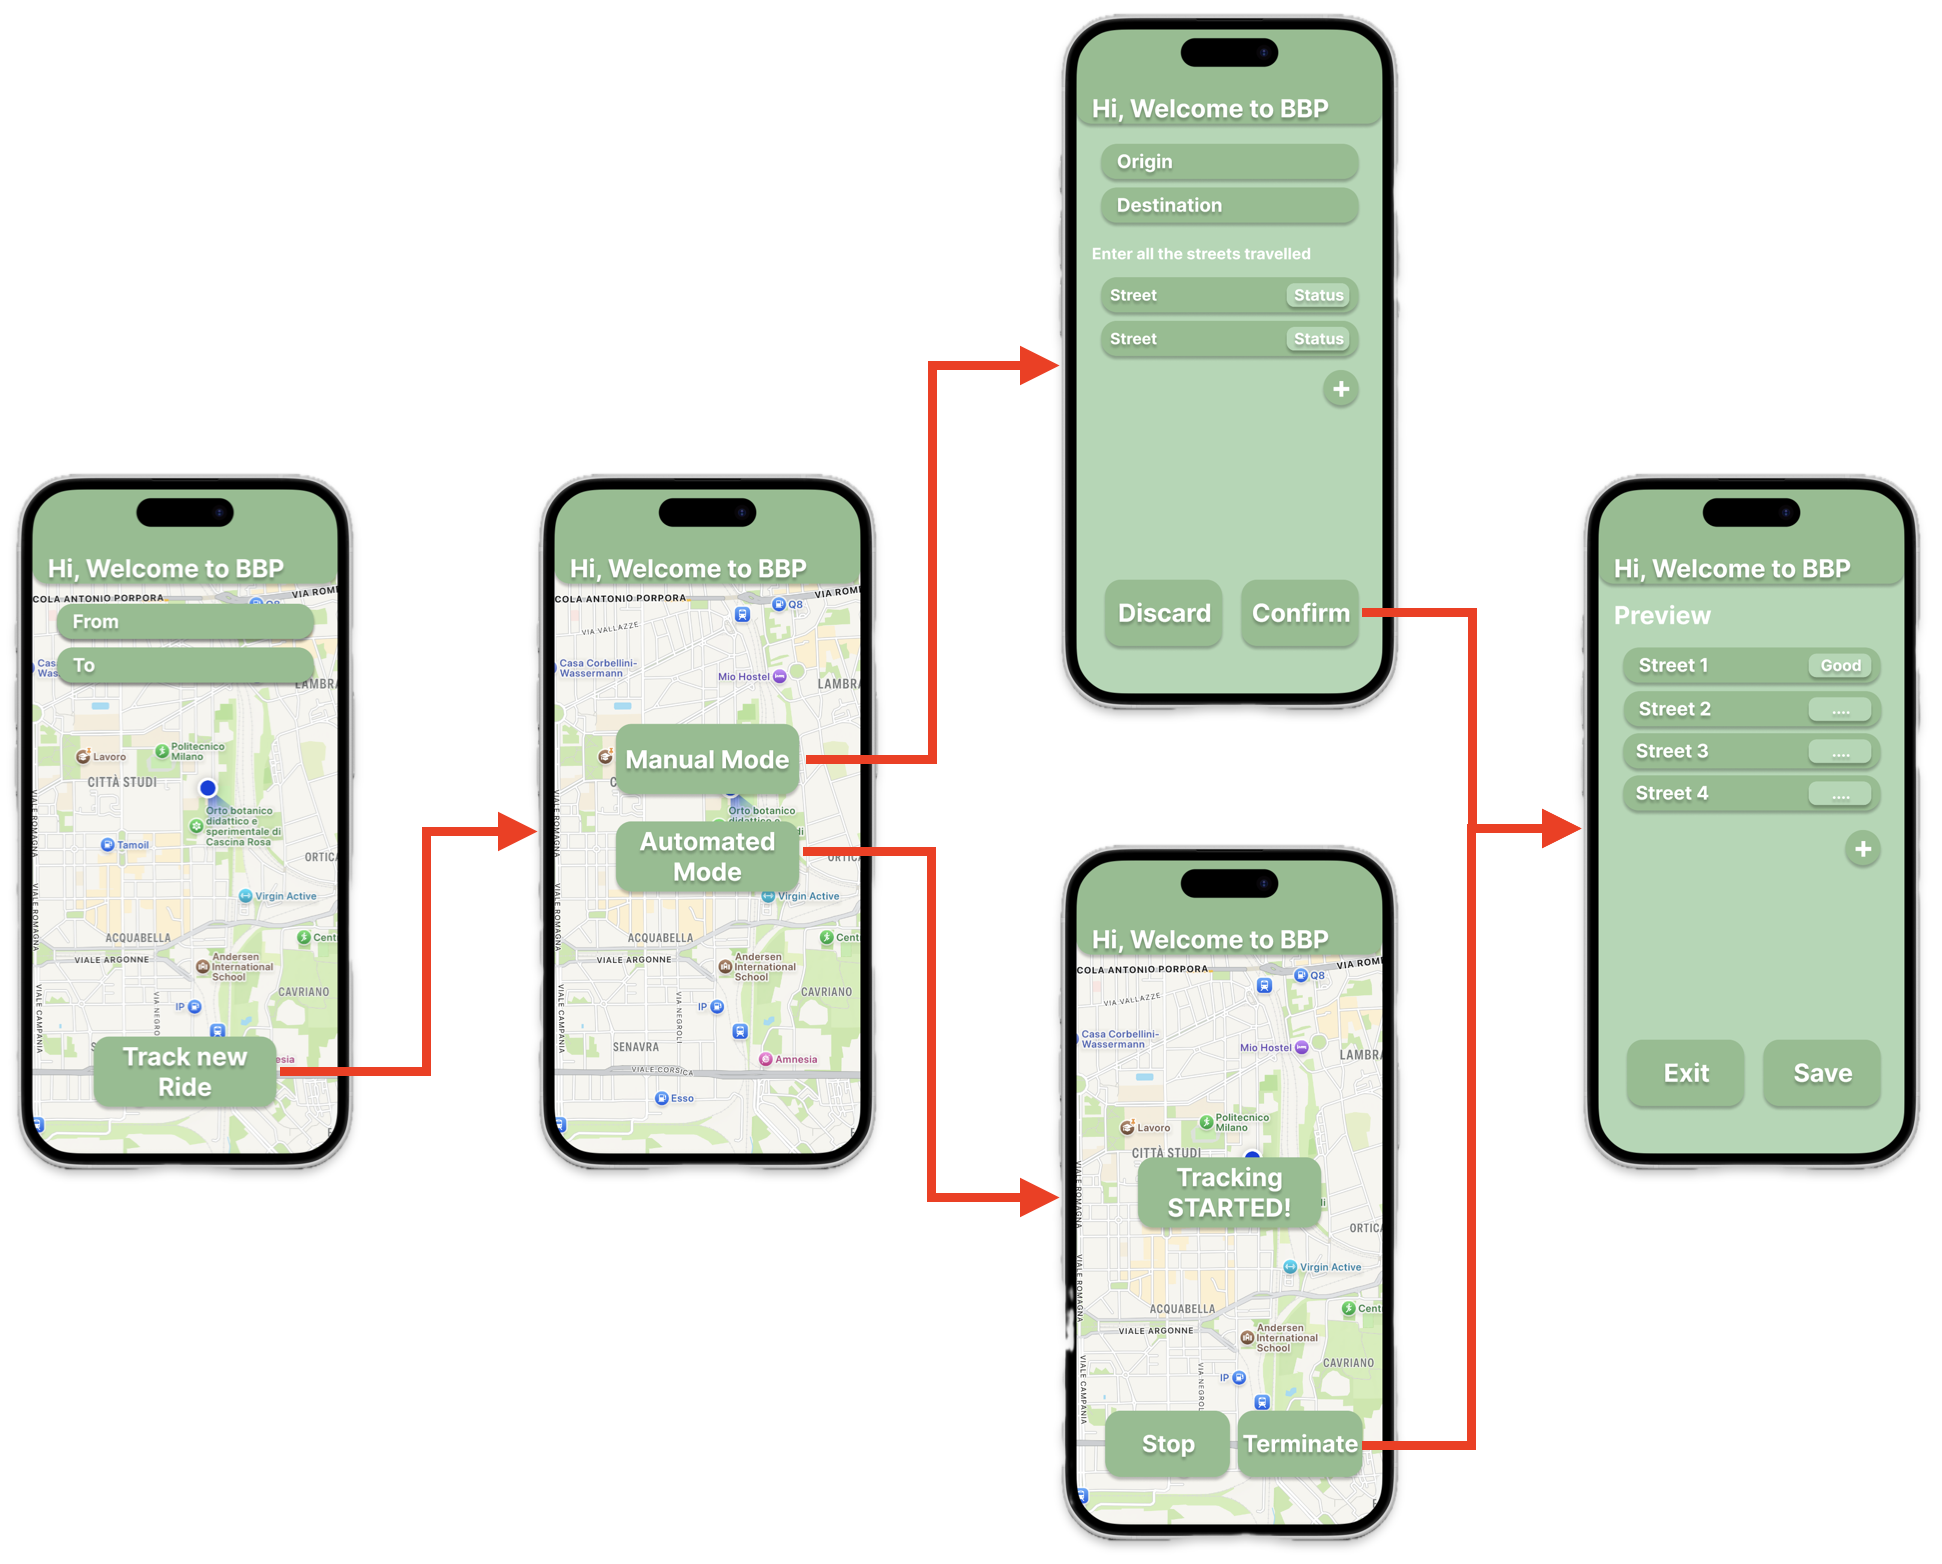
\includegraphics[width=1\textwidth]{images/prototype2.png}
    \caption{Tracking mode selection screen mockup}
    \label{fig:loggedin_mode_mockup}
\end{figure}

\noindent We now examine the automated path tracking workflow in greater detail. As can be observed, the first 
four screens are identical to those presented in the previous figure; indeed, the focus here is 
specifically on the final phase of the tracking process. In this stage, the user views the path 
preview and, after optionally refining the data, chooses to save the path, at which point they are 
presented with the option to immediately publish the record. \\

\begin{figure}[H]
    \centering
    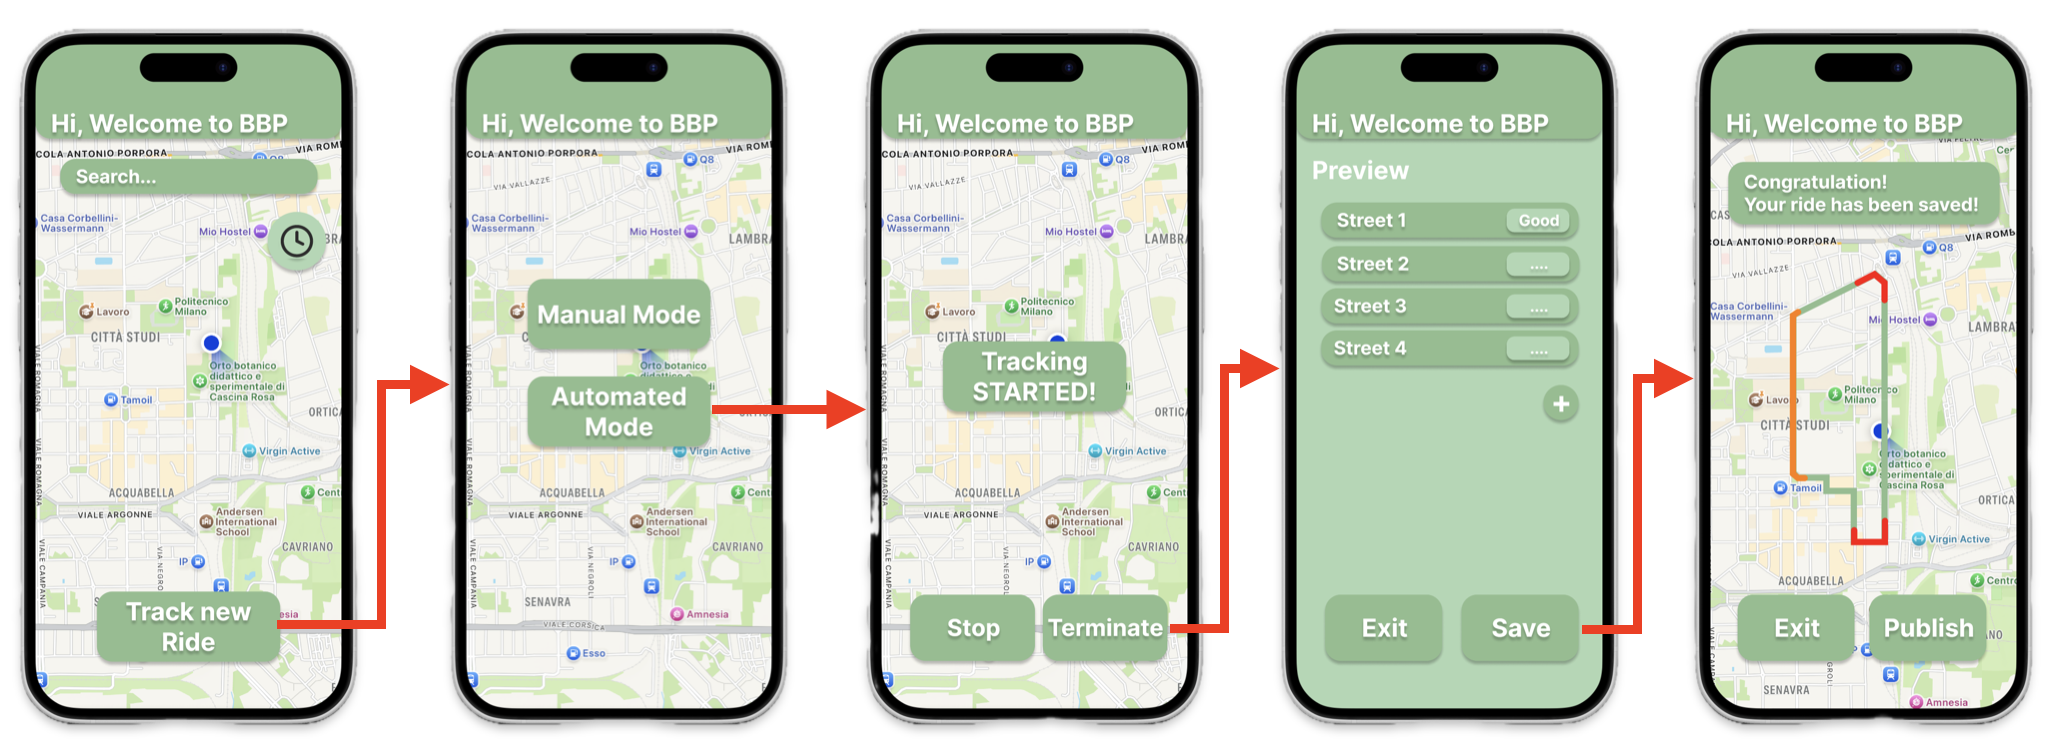
\includegraphics[width=1\textwidth]{images/prototypeAUTOMATED.png}
    \caption{Automated tracking screen mockup}
    \label{fig:Automated_tracking_mockup}
\end{figure}    

\noindent Proceeding further, we encounter the workflow for viewing a specific record within the sessions inventory. Specifically, the Home Screen features a button that grants access to the complete list of 
records. From this list, users can view the details of individual record, as depicted in the final 
screen on the right. This screen displays a hypothetical map that graphically highlights the path 
and indicates the status of its constituent streets.\\

\noindent This interface also allows users to review their performance metrics, which are obtained from the acquired data. Furthermore, within this view, the user must be provided with the option to modify the 
path's publication status (i.e., publishing a private path or reverting a public path to private
if the user no longer wishes to share it) and, if necessary, to delete the record entirely. \\

\noindent It should be noted that these mockups are purely illustrative and may not explicitly depict every detailed of the described features, especially under the design point of view.\\

\begin{figure}[H]
    \centering
    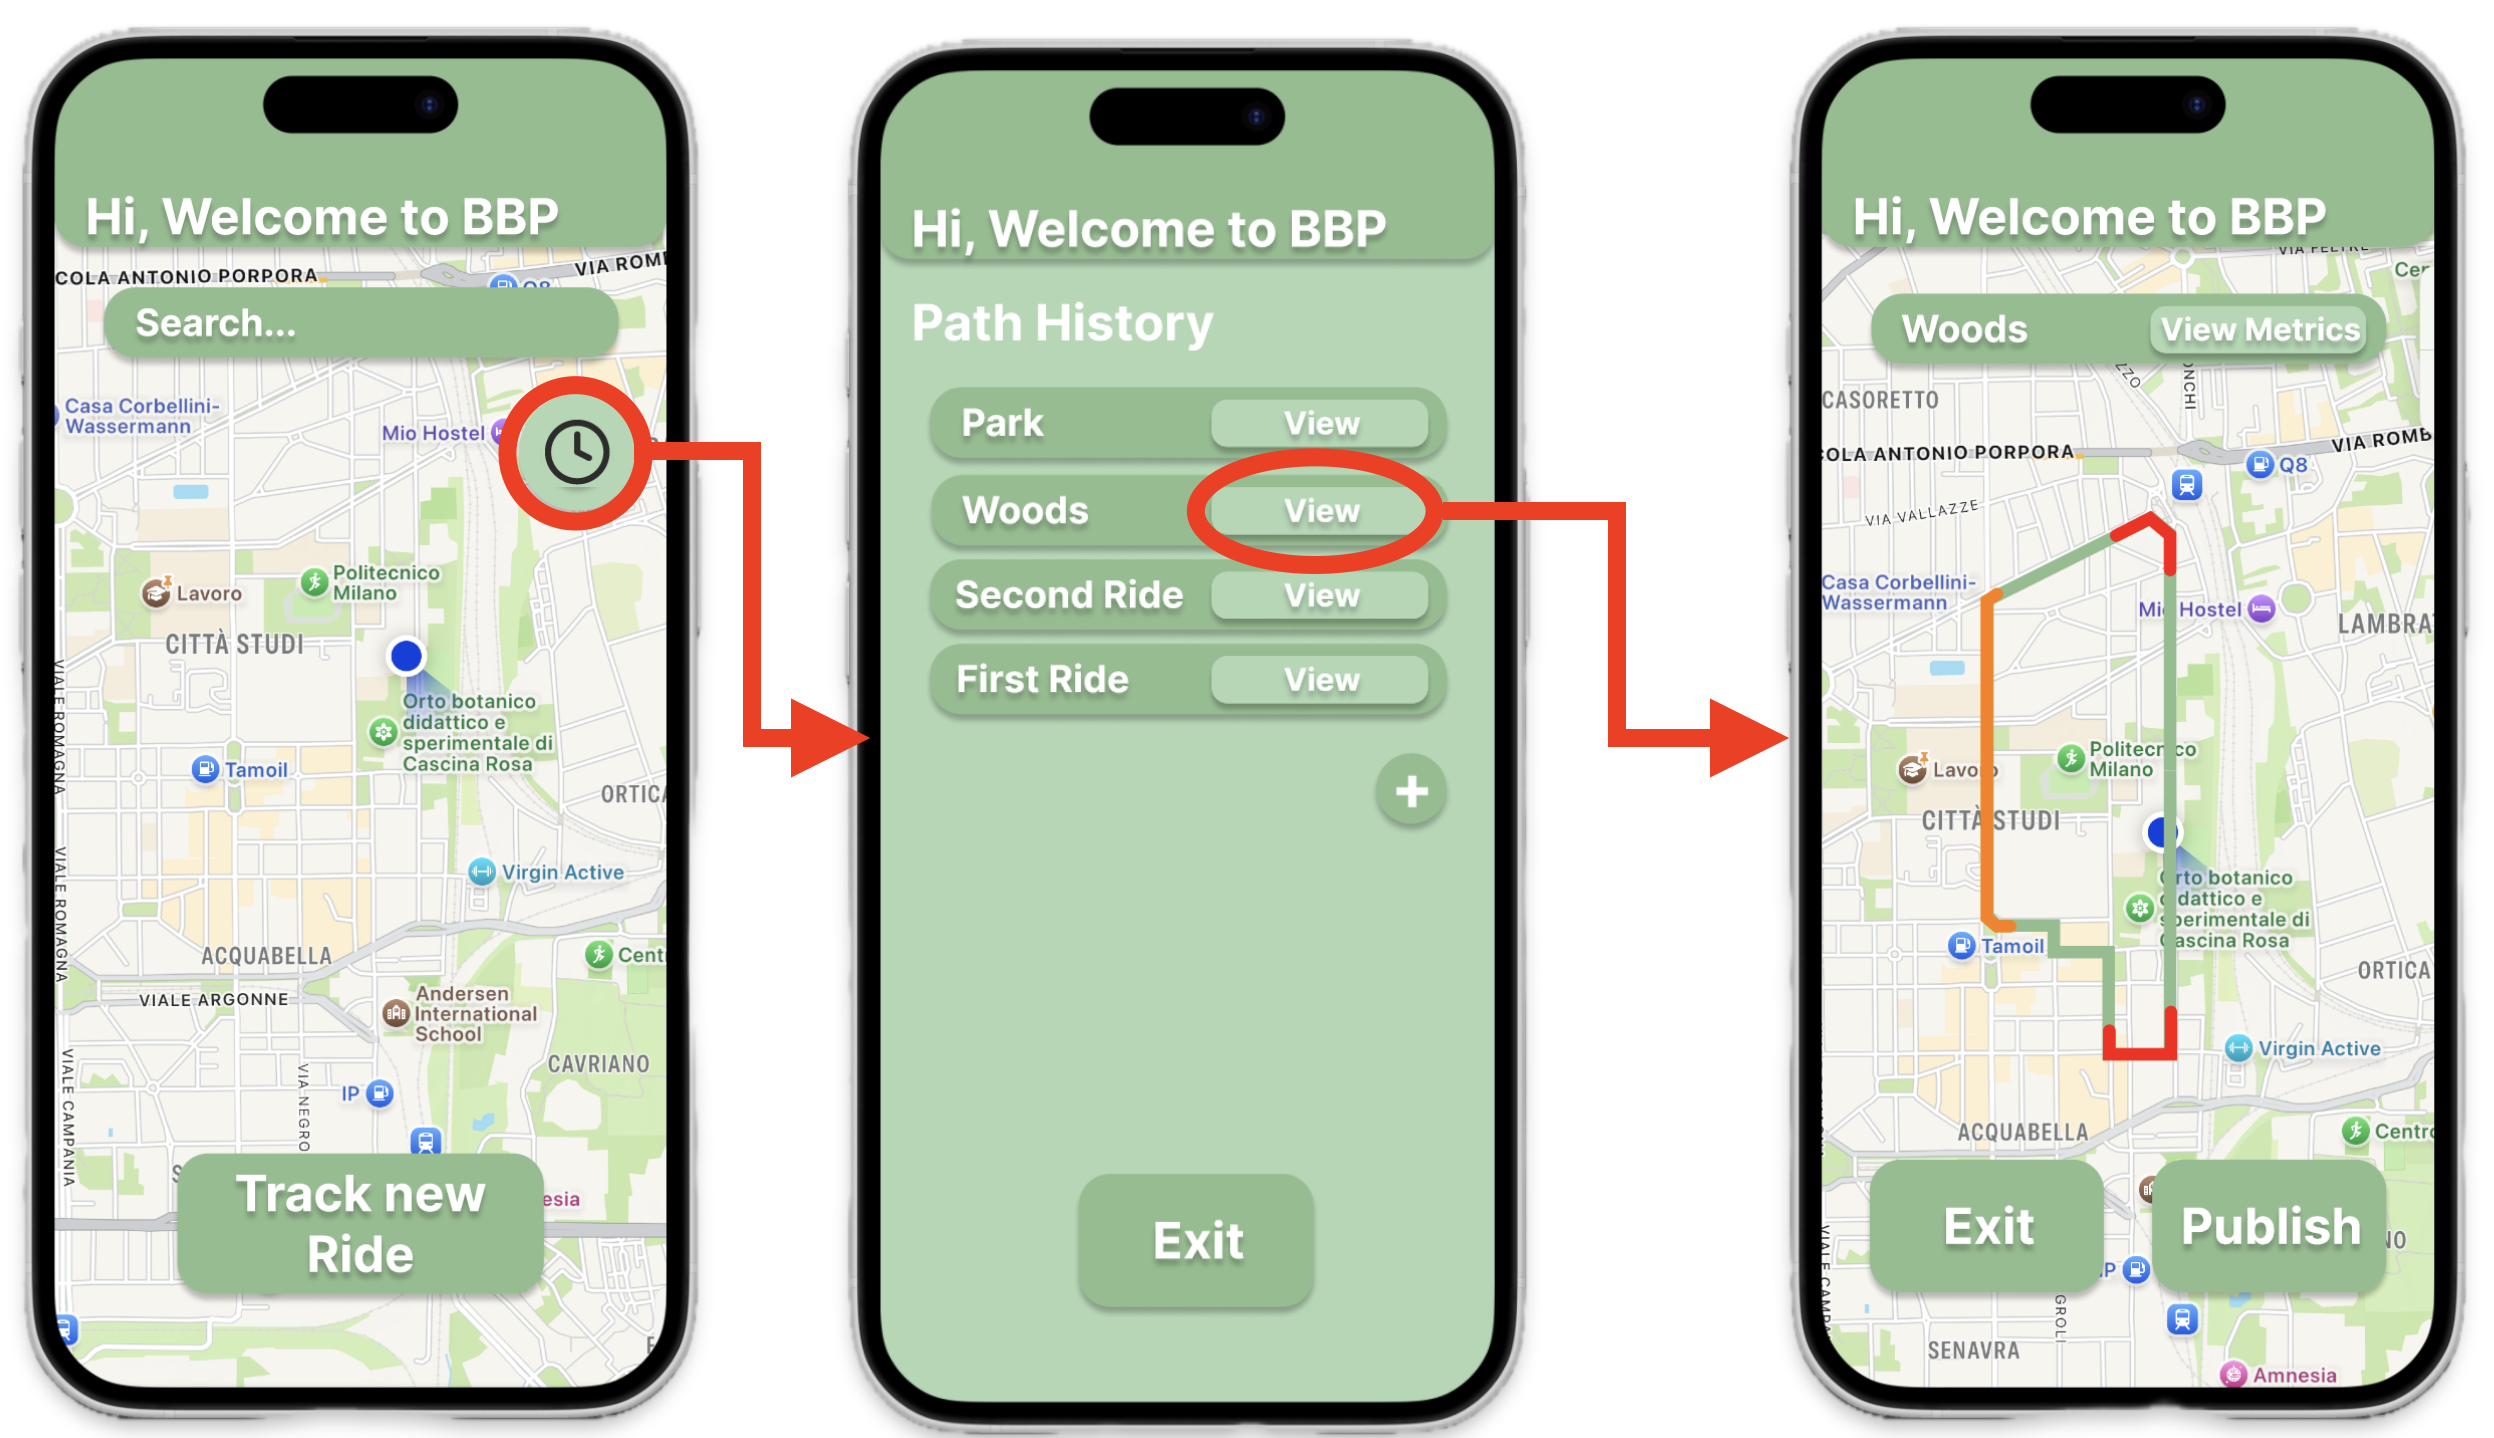
\includegraphics[width=1\textwidth]{images/prototypeVIEWRECORDS.png}
    \caption{View recorded ride screen mockup}
    \label{fig:view_recorded_ride_mockup}
\end{figure}

\noindent Finally, the last figure illustrates the path search workflow. As can be observed, the diagram 
deliberately depicts the scenario where the user is in Guest Mode. Consequently, starting from 
the main screen, the user clicks on 'Search,' enters the origin and destination, and is presented 
with a list of paths sharing similar origins and destinations, ranked by score.\\

\noindent From this list, the user has the option to press 'View' to examine the path's details and its 
associated score. It is important to note that the workflow is analogous for logged-in users. 
The primary distinction is that logged-in users, upon accessing the path detail screen, may be 
offered the option to immediately launch automatic tracking while being redirected to a third-party map application to get geographical directions; this is considered a useful but 
optional shortcut, and its inclusion is therefore left to the discretion of the implementer. \\

\begin{figure}[H]
    \centering
    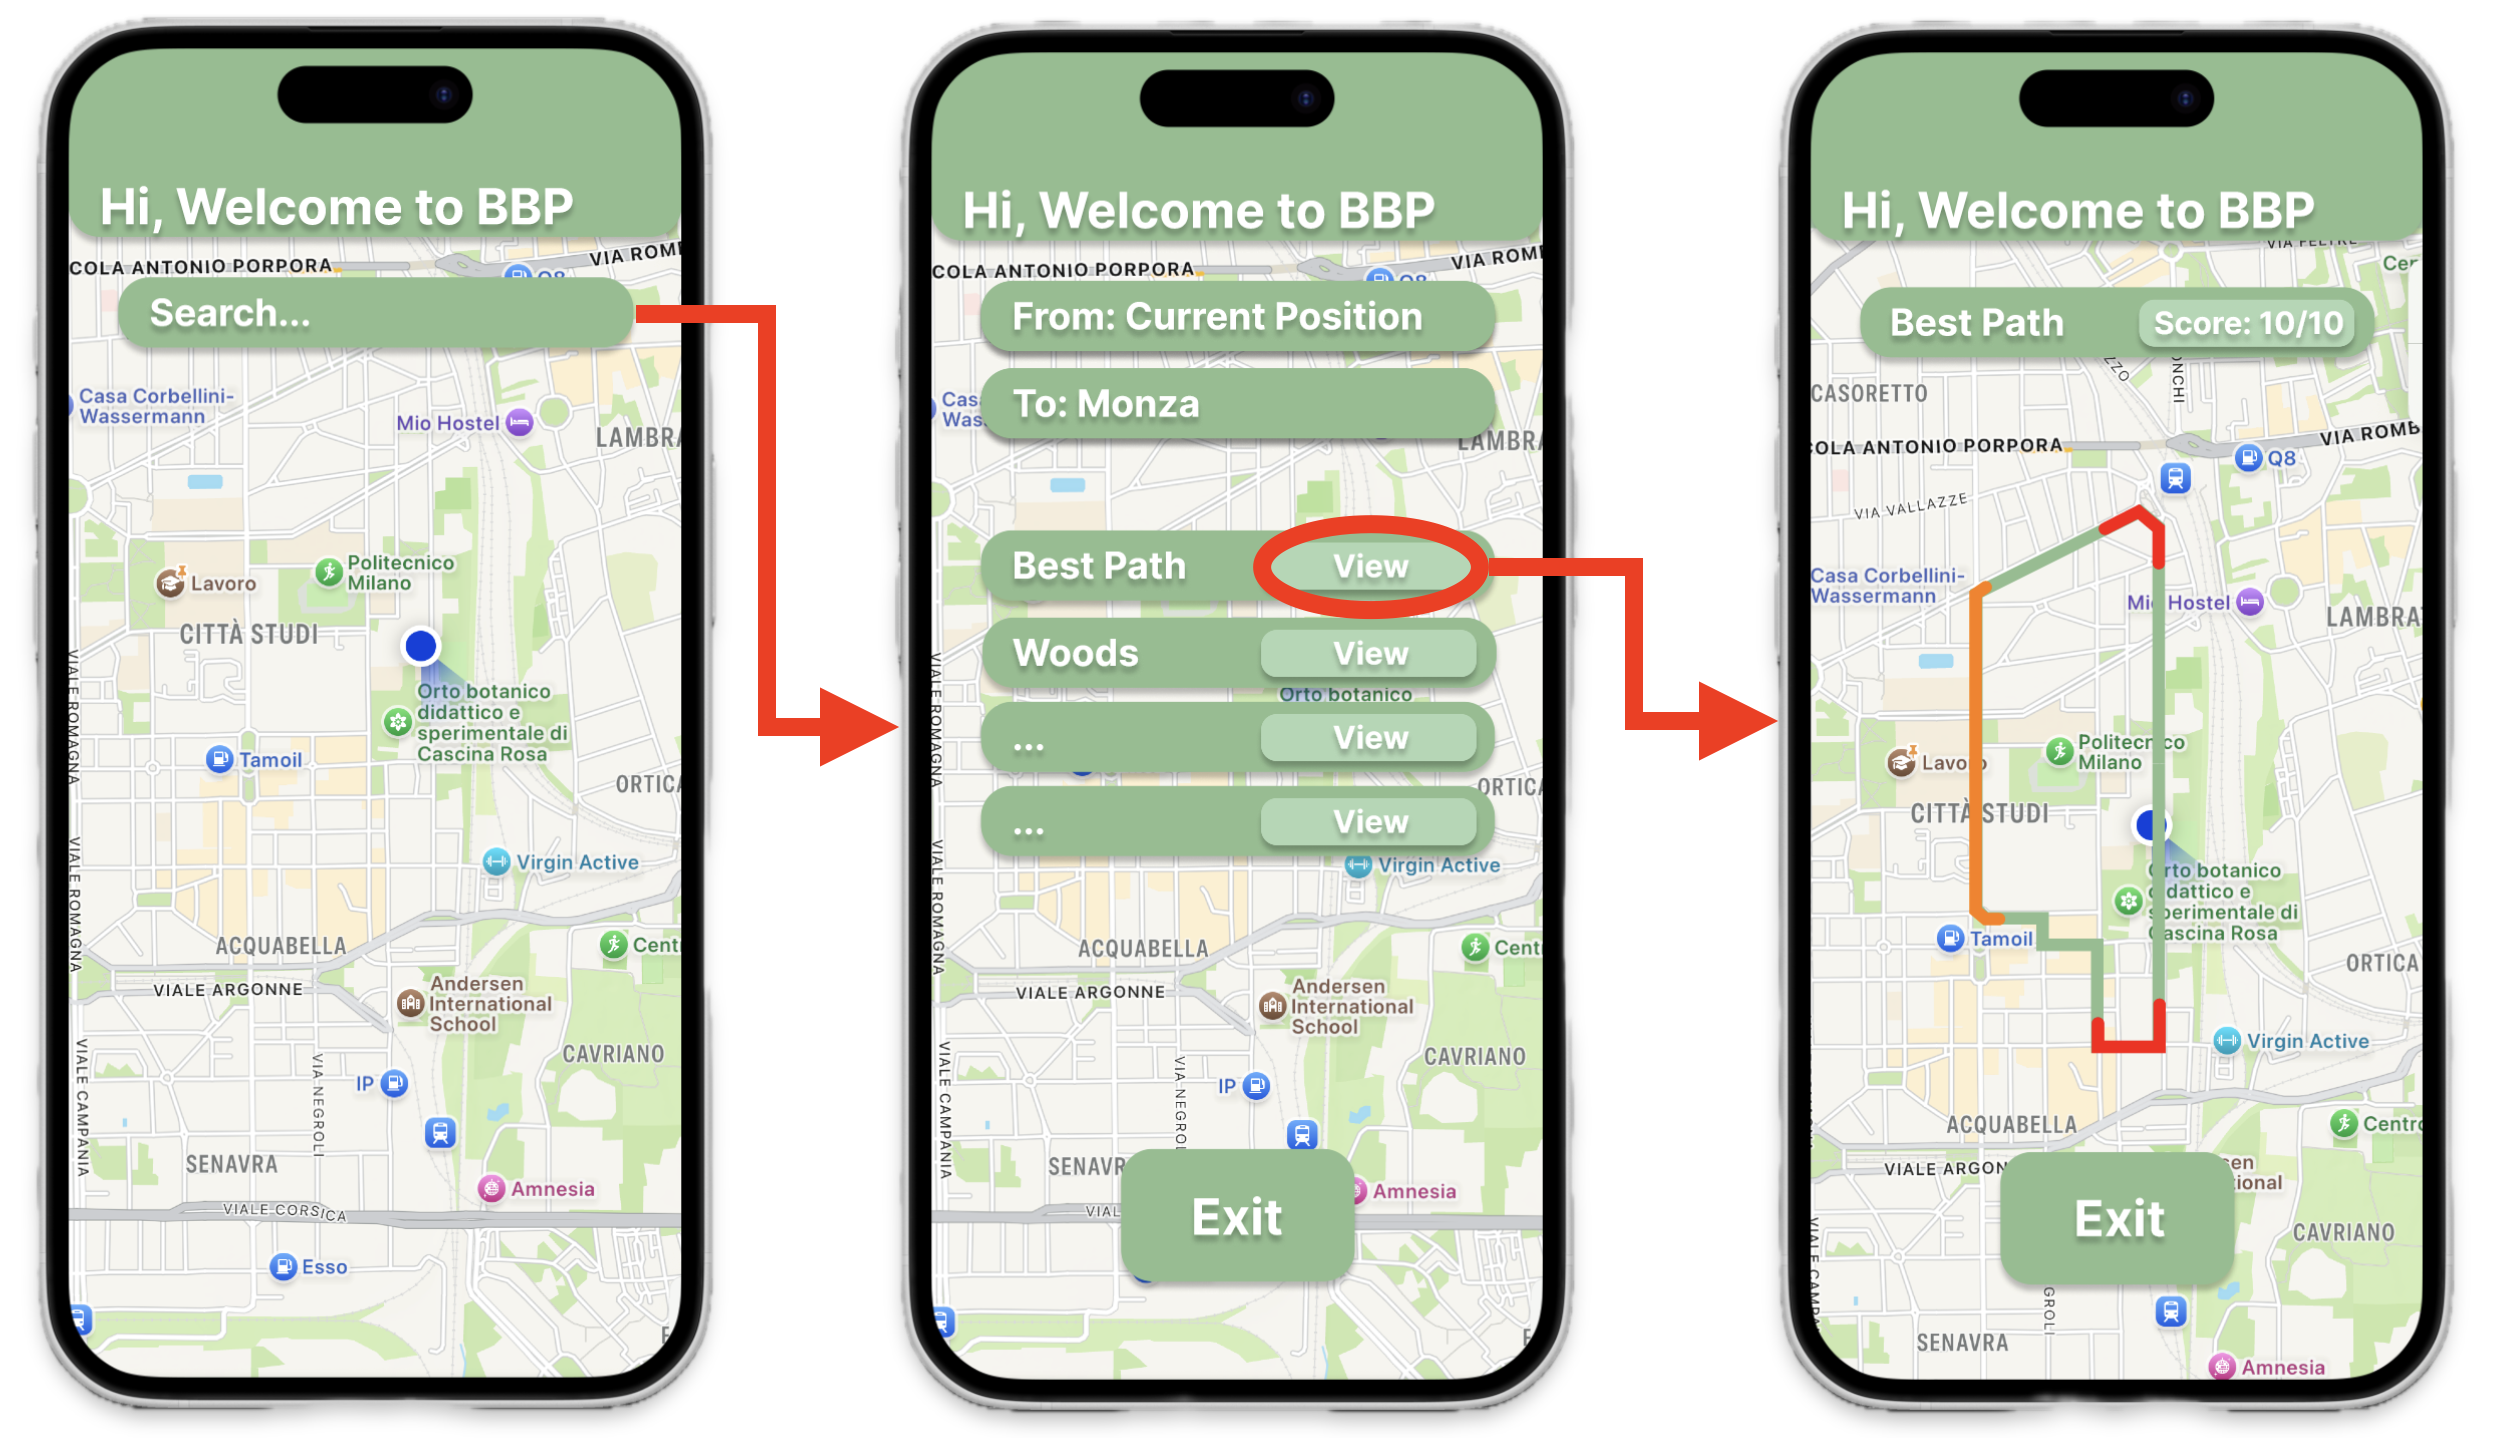
\includegraphics[width=1\textwidth]{images/prototypeSEARCHFORAPATH.png}
    \caption{Search for a bike path screen mockup}
    \label{fig:search_for_a_bike_path_mockup}
\end{figure}

\noindent It is repeated again for the sake of clarity that the mockups do not represent a strict set of guidelines to be followed in absolute terms during the implementation phase, 
but rather a starting point intended to clarify design choices and eliminate residual ambiguities.